\documentclass[a4paper]{article}
\usepackage{amsmath}
\usepackage{amsfonts}
\usepackage{amssymb}
\usepackage{booktabs}
\usepackage{graphicx}
\usepackage{enumerate}
\usepackage{xeCJK}
\usepackage{zhnumber}
\usepackage{listings}
\usepackage{float}
\usepackage[colorlinks,linkcolor=black,anchorcolor=black,citecolor=black]{hyperref}
\setCJKmainfont[BoldFont=FZHei-B01]{FZShuSong-Z01}
\setCJKfamilyfont{hei}{FZHei-B01}
\setCJKfamilyfont{kai}{FZKai-Z03}
\setCJKfamilyfont{fang}{FZFangSong-Z02}
\newcommand{\hei}{\CJKfamily{hei}}
\newcommand{\kai}{\CJKfamily{kai}}
\newcommand{\fang}{\CJKfamily{fang}}

\usepackage{fontspec}
\newfontfamily\mymono{Source Code Pro}
\usepackage{color}
\definecolor{mygreen}{rgb}{0,0.6,0}
\definecolor{mygray}{rgb}{0.5,0.5,0.5}
\definecolor{mymauve}{rgb}{0.58,0,0.82}
\lstset{
	frame=single,
	numbers=none,
	numberstyle=\footnotesize\mymono\color{mygray},
	basicstyle=\footnotesize\mymono,
	breaklines=true,
	tabsize=4,
	commentstyle=\color{mygreen},
	keywordstyle=\color{blue},
	stringstyle=\color{mymauve},
}

\title{Code Reading Report of Caffe - Version 1}
\author{计45 孟垂正 2013010952}
\date{\today}

\bibliographystyle{ieeetr}

\begin{document}
	\maketitle
	\section{Caffe简介}
	Caffe是一个基于易表达性,速度和通用性开发的深度学习框架.它由Berkeley Vision and Learning Center (BVLC)开发并由社区维护.贾扬清在UC Berkeley读博期间开创了此项目\cite{jia2014caffe}.
	
	\section{编译,安装与运行}
	本节内容主要参考官网的安装指南\cite{installationguide},同时结合了个人实践.以下操作均在Arch Linux\footnote{Arch Linux是一个通用的 i686/x86-64 GNU/Linux 发行版.Arch采用滚动升级模式,尽全力提供最新的稳定版软件.与Ubuntu不同,Arch Linux通过其包管理工具pacman安装的大部分软件包附带有必要的头文件和动态链接库,因此一般无需安装相应的libxxx-dev.}上进行,与指南中Ubuntu下的操作略有差异.
	\subsection{依赖库安装}
	Caffe主要用到的依赖库有:
	\begin{enumerate}[-]
		\item protobuf(Google出品的一种数据序列化工具)
		\item leveldb(Google出品的一种键值存储工具)
		\item snappy(Google出品的一种快速压缩/解压缩工具)
		\item opencv(著名的计算机视觉计算库)
		\item hdf5-serial(支持多种数据类型的数据组织结构和文件格式)
		\item boost(著名C++增强库)
		\item protobuf-compiler(protobuf的编译器)
		\item BLAS(可从atlas. OpenBLAS或者MKL中选择一种,以下以atlas为例)
		\item gflags(提供命令行参数管理功能的库)
		\item glog(提供Log功能的库)
		\item CUDA(可选,NVIDIA显卡的GPU计算库,若CPU-only则无需安装)
		\item Python(可选,若需要Caffe的Python接口)
	\end{enumerate}
	Arch Linux下的安装指令为:
	\begin{lstlisting}[language=bash]
sudo pacman -S protobuf leveldb snappy opencv hdf5 boost boost-libs
sudo pacman -S atlas-lapack-base
sudo pacman -S gflags google-glog
sudo pacman -S cuda python
	\end{lstlisting}
	\subsection{编译与安装}
	从https://github.com/BVLC/caffe.git获取源码并切换到对应目录.
	\begin{lstlisting}[language=bash]
cd ~
git clone https://github.com/BVLC/caffe.git
cd ./caffe
	\end{lstlisting}
	修改配置文件并进行编译.如需要开启CUDNN,开启CPU-only模式,更改默认BLAS库(atlas)或者使用Python接口,在Makefile.config中参照注释进行必要修改即可.
	\begin{lstlisting}[language=bash]
cp Makefile.config.example Makefile.config
# Adjust Makefile.config (for example, if using Anaconda Python, or if cuDNN is desired)
make all -j4
make test
make runtest
	\end{lstlisting}
	runtest结束后可检验安装是否成功.
	\subsection{运行Demo}
	安装成功后可尝试运行Caffe附带的LeNet Demo.LeNet-5\cite{lecun2015lenet}是由Y.LeCun等人设计的用于识别手写和打印字符的卷积神经网络.其主要结构如下图:
	\begin{figure}[H]
		\centering
		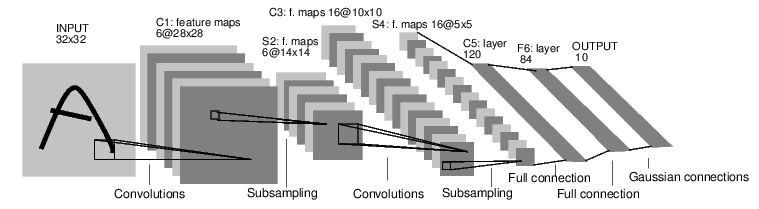
\includegraphics[width=\linewidth]{lenet5.png}
		\caption{LeNet-5的结构图}
		\label{lenet5}
	\end{figure}
	切换到caffe根目录并执行脚本获取数据集.然后执行脚本进行训练.
	\begin{lstlisting}[language=bash]
cd ~/caffe
./data/mnist/get_mnist.sh
./examples/mnist/create_mnist.sh
./examples/mnist/train_lenet.sh
	\end{lstlisting}
	最终结果如下图.
	\begin{figure}[H]
		\centering
		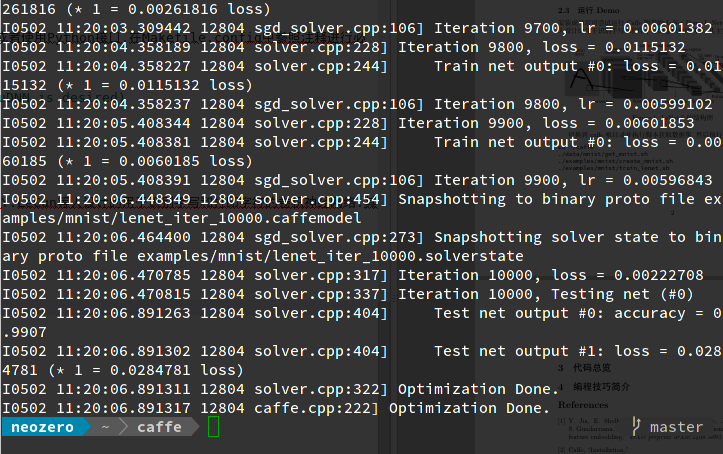
\includegraphics[width=\linewidth]{lenetresult.png}
		\caption{LeNet的训练结果}
		\label{training}
	\end{figure}
	
	\section{系统总览}
	Caffe是一个用于搭建深度神经网络的框架.为了了解其功能,此处有必要对深度神经网络做简要的介绍.
	\subsection{深度神经网络}
	深度神经网络是在神经网络的基础上发展而来.由于篇幅限制,此处对神经网络不再过多介绍,读者如有需要可参考任何一本机器学习/人工智能/数学建模方面的基础书籍.概括而言,初级的神经网络接受$n$个变量的输入,经过输入层-隐层-输出层的路径,在各层的权重和激励函数作用下得到$m$个输出变量.而训练目标即为求解最优的权重值组合使得输出与真实值之间的误差最小.\\\\
	现实应用中,这种简单的神经网络结构表现的好坏与输入的选择密切相关.以围棋为例,若欲训练出一神经网络,使之接受当前局面并输出下一步落子位置,则简单地将<所有棋盘位置上的落子情况,下一步落子位置>组成的训练数据作为输入将不能得到理想的结果.在深度学习出现之前,通常需要人类专家结合先验知识进行输入的合理选择和设计(称为"feature engineering")\cite{zhouzhmldeeplearning},而这并不容易.\\\\
	深度学习的出现,使得特征学习成为可能.典型的深度学习模型,即为很多层的神经网络(存在多个隐层),若采用BP神经网络的训练方法,计算开销将无法忍受,并且计算结果常常会发散而无法达到稳定.一种节省开销的方法为CNN(卷积神经网络),例如Figure \ref{lenet5}中的LeNet-5.网络的输入为图像的各个像素灰度值,经过多个卷积层-采样层对输入进行加工后得到卷积层数据,最后输入到一个普通神经网络进行输出.在训练过程中,同一层的每个神经元均采用相同的权值,从而需要计算的参数数目大幅减少.
	\subsection{Caffe提供的功能}
	作为一个深度学习框架,Caffe提供了以下基本功能来帮助使用者较容易地搭建自己的深度神经网络.
	\begin{enumerate}
		\item 易于编辑的表达方式\ 模型和优化算法均用纯文本(.protobuf)定义而非固化在代码中.
		\item 高速计算\ 支持使用GPU加速计算.
		\item 扩展性\ 使用者可方便地根据需求添加自己需要的扩展功能.
	\end{enumerate}
	\section{系统结构设计}
	Caffe实现了建模与求解的解耦,故其系统结构可从这两方面分析.
	\subsection{建模}
	建模方面,Caffe采用的网络结构范式为:Blob-Layer-Net三层结构.
	\begin{enumerate}
		\item Blob.Blob为Caffe中数据的基本单元,以数组形式存储数据,提供底层的内存管理功能.
		\item Layer.Layer对应深度神经网络中"层"的概念,是构成整个网络的基础构件,进行网络中的计算与数据处理.
		\item Net.Net是多个Layer的组合,管理网络中各层的连结关系.
	\end{enumerate}
	\subsection{优化}
	求解方面,Caffe实现了SGD(Stochastic Gradient Descent)等常用优化方法,从Net中接收当前的代价函数和梯度,输出各参数的更新量.求解器还提供检验训练效果和保存训练阶段性成果的功能.
	
	\section{数据设计}
	Caffe通过Blob-Layer-Net三层结构存储输入数据和配置文件,使用Solver对模型进行优化求解.
	\subsection{数据描述}
	由于神经网络的结构差异很大,为尽可能简单地说明功能,以单层感知机为例说明Caffe处理数据的流程.
	\begin{figure}[H]
		\centering
		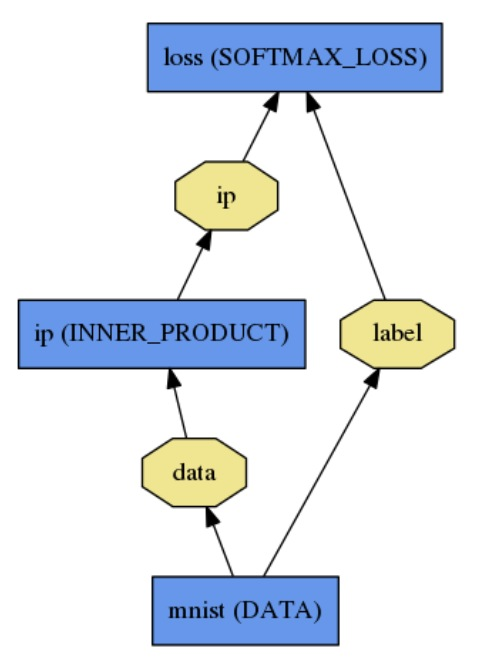
\includegraphics[width=0.3\linewidth]{logreg.jpg}
		\caption{单层感知机在Caffe中的结构示意图\cite{caffebln}}
		\label{logreg}
	\end{figure}
	\subsubsection{外部数据输入网络}
	Caffe采用一种专门的Layer-DataLayer进行数据的读取.通过使用相关库,Caffe支持读取leveldb/lmdb等数据库,内存数据,HDF5类型数据和图片格式数据.使用时通过protobuf配置文件为DataLayer设置2个top Blob(data和label)作为该层的输出.Figure \ref{logreg}中底部的mnist层即为DataLayer.\\\\
	DataLayer通过内部的DataReader类将数据读进内存并传入输出Blob.DataReader类通过一个map为每个数据源维护一个用于读取此数据源的Body.每个Body为当前需要该数据源的所有Net维护一个QueuePair队列,其中QueuePair同样是一个队列,用于依次存放解析得到的数据.Body内部开启一个主循环线程将数据不断读入每个网络所在的队列.如此设计主要原因是适应同时训练多个网络的情况.\\\\
	当一个Net中的DataLayer需要读取数据时,它通过map寻找到读取所需数据源的Body,并从相应队列中取出数据,根据数据种类将其分为data和label并分别传至top的Blob中.
	\subsubsection{数据在网络中的流动}
	除了数据层外,Net中的每一个Layer均需定义其输入(bottom Blobs)和输出(top Blobs).Figure \ref{logreg}中的ip层(全连接层)的输入为data,输出为ip.有必要注意的是,Layer内部同样采用Blob存储网络权重等结构信息.\\\\
	每个Layer需要实现2类函数:Forward和Backward(实际上每类还要分为cpu和gpu,此处只讨论cpu编程),分别对应BP神经网络的前向传播和反向传播.这类函数中,Layer通过Blob提供的接口获取其中数据的指针并进行运算.以Forward函数为例,其形式一般为$f\left(X,W,Y\right)$,其中$X$为bottom Blob的数据,$W$为Layer中的权重,偏移量等数据,$Y$为输出数据.$f\left(X,W,Y\right)$为矩阵运算函数,Caffe在此处直接调用安装时指定的BLAS库接口进行计算.\\\\
	为了适应不同的传播函数,Caffe在此处大量运用了C++的继承和多态特性,也为使用者开发自己需要的Layer提供了方便.开发者需要继承Layer类并实现其中的初始化,正/反向传播函数.
	\subsubsection{数据从网络中输出}
	Solver的配置文件中可设置每过一定的训练间隔即可将当前最优的网络保存.Solver将Net中所有Layer的权重和连接关系保存为二进制文件以便于使用和继续训练.
	
	\section{用户接口}
	Caffe提供了可执行程序caffe用于网络的训练,检验和时间测试.进行训练的结果见Figure \ref{training}.
	\begin{lstlisting}[language=bash]
# train LeNet
caffe train -solver examples/mnist/lenet_solver.prototxt
# score the learned LeNet model on the validation set as defined in the
# model architeture lenet_train_test.prototxt
caffe test -model examples/mnist/lenet_train_test.prototxt -weights examples/mnist/lenet_iter_10000.caffemodel -gpu 0 -iterations 100
# time LeNet training on CPU for 10 iterations
caffe time -model examples/mnist/lenet_train_test.prototxt -iterations 10
	\end{lstlisting}
	Caffe也提供了Python接口,需要编译pycaffe并安装.
	
	\section{编程技巧}
	\subsection{继承与多态的运用}
	OOP中的继承与多态在Caffe中得到大量运用.以Layer类为例,其中LayerSetup(),Reshape(),Forward(),Backward()等成员函数均设置为虚函数.由于神经网络中Layer用到的运算繁多,因此需要借助虚函数在其子类中实现各种运算.这一特性也方便了新Layer的开发,增强了系统的通用性.
	\subsection{拷贝构造函数和赋值运算符的禁用}
	在caffe/common.hpp中Caffe通过宏的形式禁用了某些类的拷贝构造函数和赋值运算符.
	\begin{lstlisting}[language=C++]
// Disable the copy and assignment operator for a class.
#define DISABLE_COPY_AND_ASSIGN(classname) \
private:\
  classname(const classname&);\
  classname& operator=(const classname&)
	\end{lstlisting}
	通过禁用二者可以使得所有以该类为参数的函数采用传引用方式,避免了传值方式带来的额外开销,对于Caffe中内部存储较多数据的结构其意义更为明显.
	\subsection{命名空间的合理使用}
	在头文件中使用命名空间很容易造成其使用的混乱,例如:
	\begin{lstlisting}[language=C++]
// header.h
...
using namespace caffe;
...
	\end{lstlisting}
	多次include之后将难以确定某段代码所使用的命名空间.但完全不使用命名空间会造成很多不方便,因此Caffe采用限定其作用域的方法解决这一问题.
	\begin{lstlisting}[language=C++]
// header.h
...
namespace caffe {
    ...
} // namespace caffe
	\end{lstlisting}
	
	\bibliography{code_reading_caffe}
	
\end{document}